% !TEX root = ../rapport.tex
\chapter{Simulations et r\'esultats}\label{simu}

\section{Outils de programmation}
Nos contraintes d'implémentation lors de ce TER étaient d'utiliser le simulateur de réseaux \href{http://wsnet.gforge.inria.fr/}{WSNET}. Ce simulateur (décrit comme un "simulateur évènementiel pour les grands réseaux de capteurs sans fils") est constitué d'un ensemble de modules en langage $C$. Ces modules correspondent aux différentes couches réseaux (voir figure \ref{structWSNET}).
\begin{figure}[h]
\centering
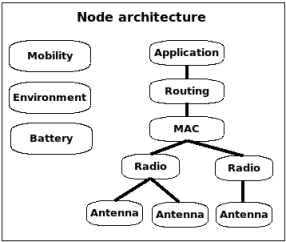
\includegraphics[scale=1]{Simus/wsnet-node}
\label{structWSNET}
\end{figure}
Cette bibliothèque est développée par trois chercheurs lyonnais : Guillaume Chelius, (chercheur INRIA), Antoine Fraboulet (maitre de conférence) et Elyes Ben Hamida (doctorat).

Dans le cadre de notre TER, nous avons développé onze modules supplémentaires pour WSNET : 
\begin{itemize}
	\item un module utilitaire contenant des structures de données
	\item un module gérant la consommation énergétique
	\item un module gérant la couche liaison (protocole mac) sans interférences mais qui appelle le module de consommation d'énergie
	\item sept modules de routage (le cœur de notre TER)
		\begin{itemize}
			\item uni-cast : Flow Augmentation \cite{Chang2000}
			\item diffusion aveugle
			\item RBOP \cite{Cartigny2005}
			\item LBOP \cite{Cartigny2005}
			\item BIP \cite{Wieselthier2000}
			\item LBIP \cite{Ingelrest2008}
			\item DLBIP \cite{Champ2009DLBIP}
		\end{itemize}
	\item un module gérant la couche application et permettant la diffusion depuis plusieurs sources
\end{itemize}
~\\
Nous avons également écrit différents scripts $bash$ et $C++$ afin d'automatiser les phases de tests ainsi que la collecte des résultats. Enfin, nous avons développé un visualisateur de graphes sous \href{http://qt.nokia.com/}{Qt} afin de pouvoir vérifier la pertinence de nos résultats sur une topologie donnée.


\section{Paramètres de simulation}

À l'aide de tous ces outils, nous avons pu nous lancer dans les simulations des différents algorithmes de routage. Pour cela, nous avons fixé différents paramètres :

\renewcommand\arraystretch{1.6}
\begin{tabular}{| l | c |}
\hline
nombre de capteurs (nœuds du graphe) & $100$ \\ \hline
rayon d'émission maximum & $30m$ \\ \hline
taille de la zone où sont répartis les capteurs & $1000 \times 1000 m^2$ \\ \hline
durée de simulation & $10000s$ \\ \hline
temps entre deux diffusions & $2s$ \\ \hline
\end{tabular}

Ces paramètres sont communs à toutes nos simulations. Cependant, certains autres paramètres varient : la topologie du réseau, les constantes $\alpha$ et $c$ du modèle énergétique et la quantité d'énergie initiale des nœuds.


\section{Topologie aléatoire}
Ces phases de test ont été effectuées en utilisant un générateur de graphes aléatoires connexes que nous avons écrit en C++. Cette topologie permet de se rapprocher au mieux du contexte général des réseaux de capteurs.

Le modèle énergétique que nous avons choisi d'utiliser fixe la consommation énergétique lors de l'envoi d'information à $ r^\alpha + c $. Nous avons lancé deux phases de tests avec des valeurs différentes pour les constantes $\alpha$ et $c$.

\subsection{Modèle énergétique simple}
Le modèle énergétique le plus simple (mais aussi le plus éloigné de la réalité) utilise les valeurs suivantes pour les constantes énergétiques : $\alpha = 2$ et $c = 0$.

\subsubsection{Time To First Fall}
\begin{bigcenter}
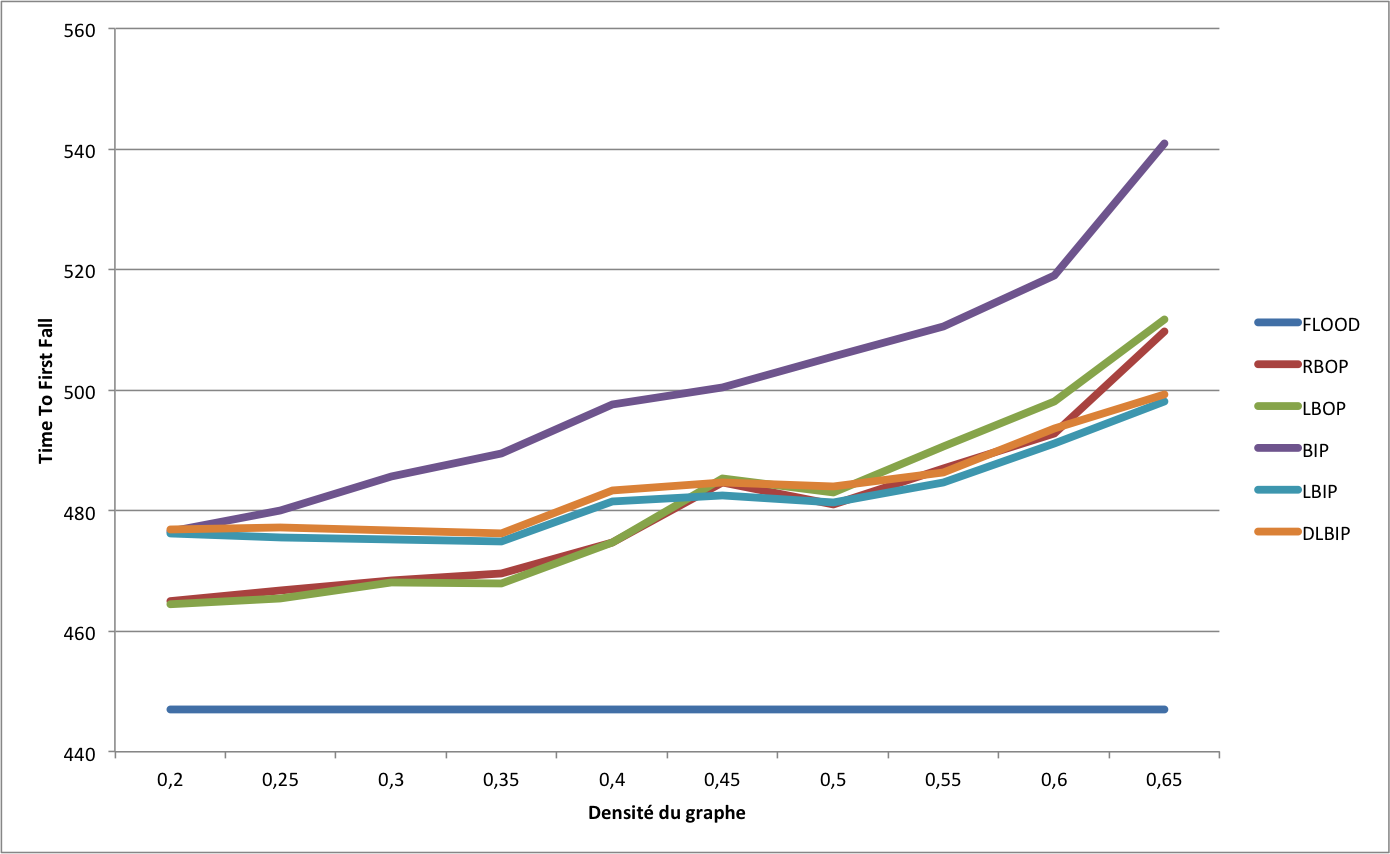
\includegraphics[scale=0.89]{Simus/ttff_2_0}
\end{bigcenter}


\subsubsection{PerCent Node}
\begin{bigcenter}
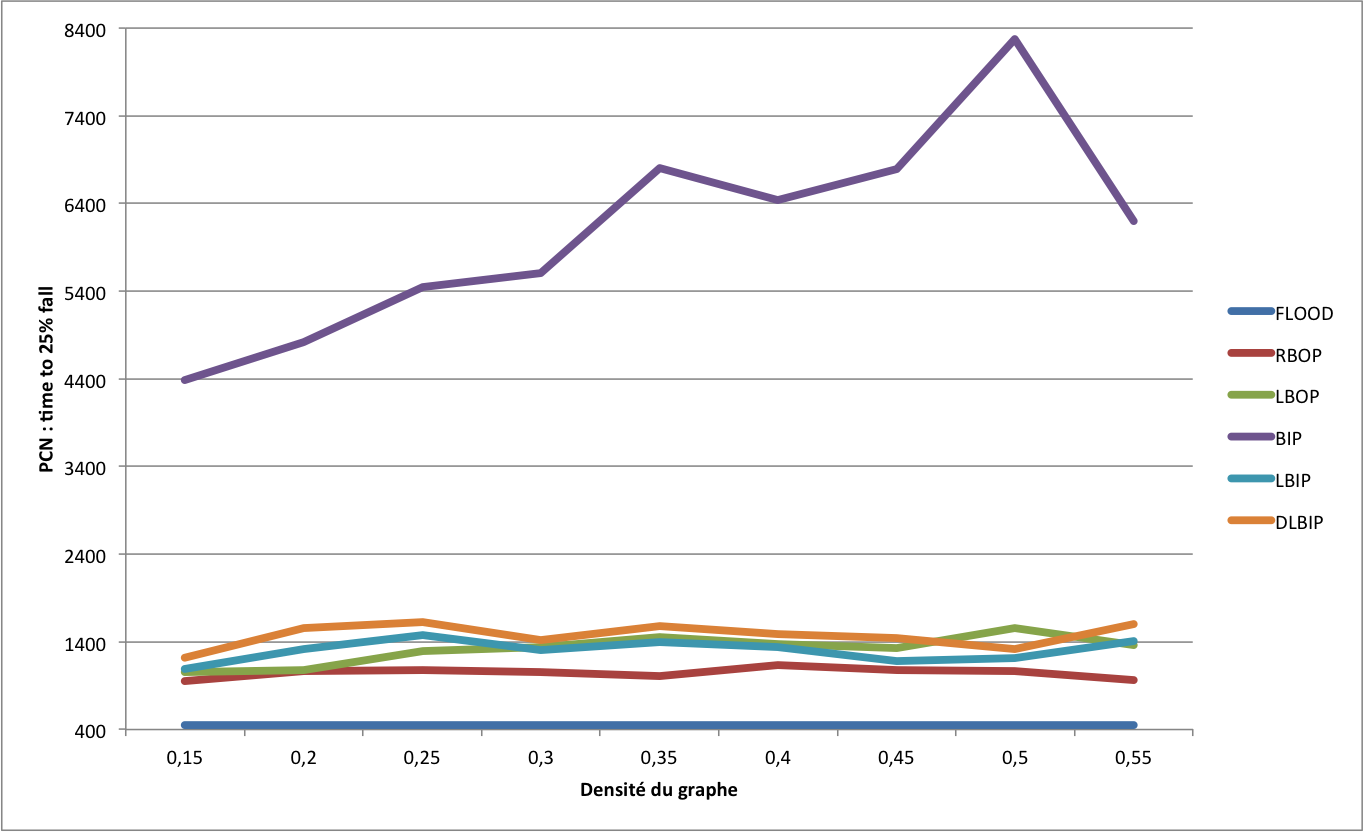
\includegraphics[scale=0.9]{Simus/pcn_2_0}
\end{bigcenter}

\begin{bigcenter}
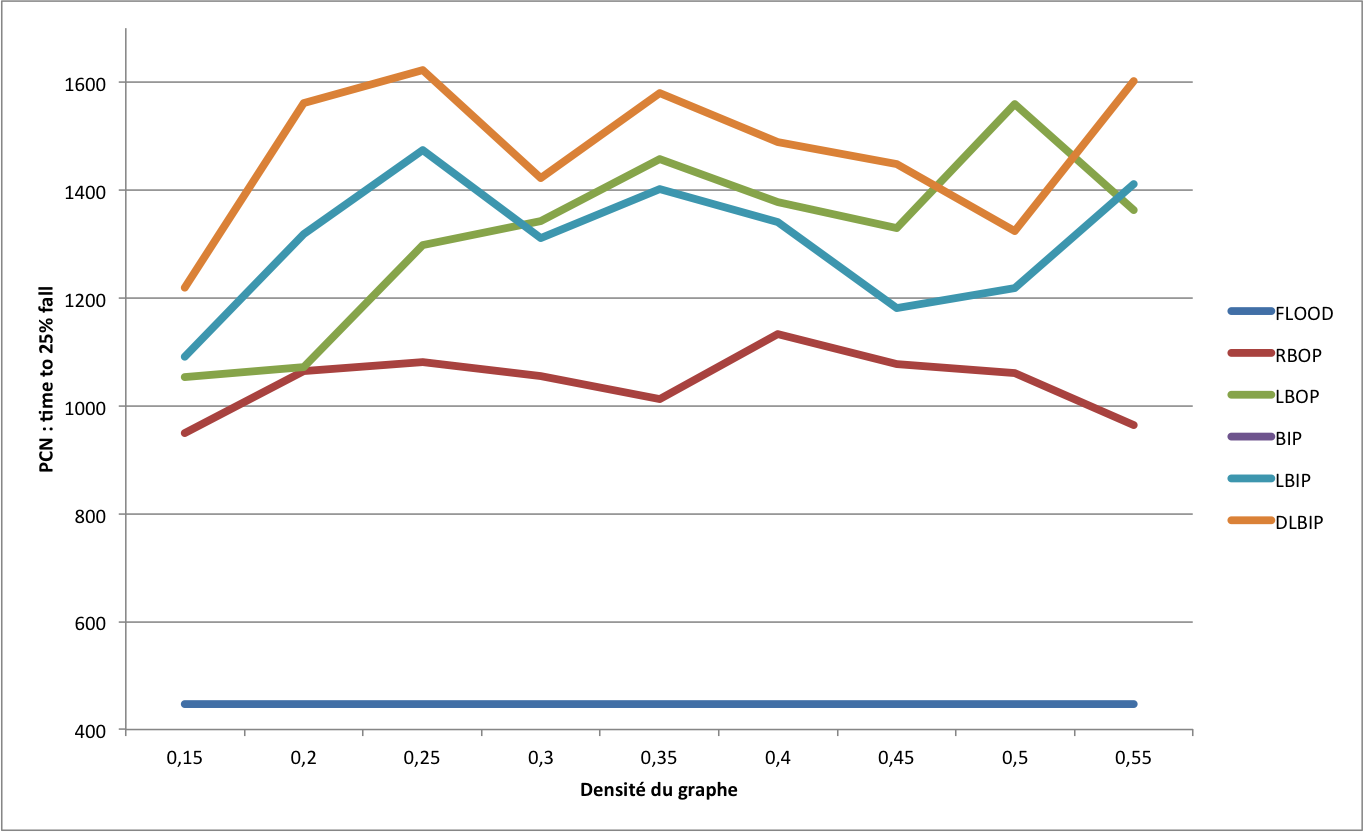
\includegraphics[scale=0.9]{Simus/pcn_2_0_zoom}
\end{bigcenter}


\subsubsection{Lose Connectivity}
\begin{bigcenter}
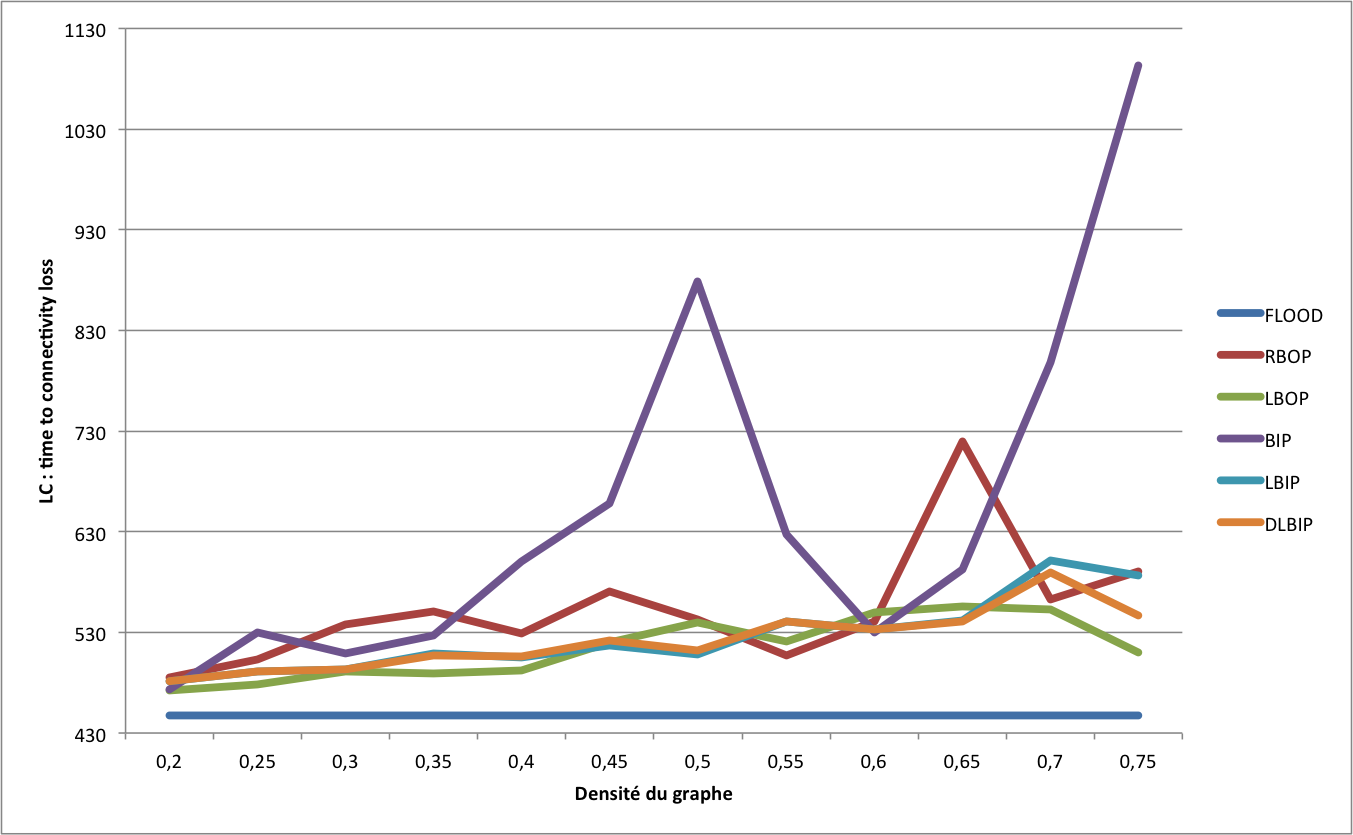
\includegraphics[scale=0.91]{Simus/lc_2_0}
\end{bigcenter}


\subsection{Modèle énergétique plus réaliste}
Ce modèle énergétique un peu plus réaliste utilise les valeurs suivantes pour les constantes énergétiques : $\alpha = 4$ et $c = 10^6$.

\subsubsection{Time To First Fall}
\begin{bigcenter}
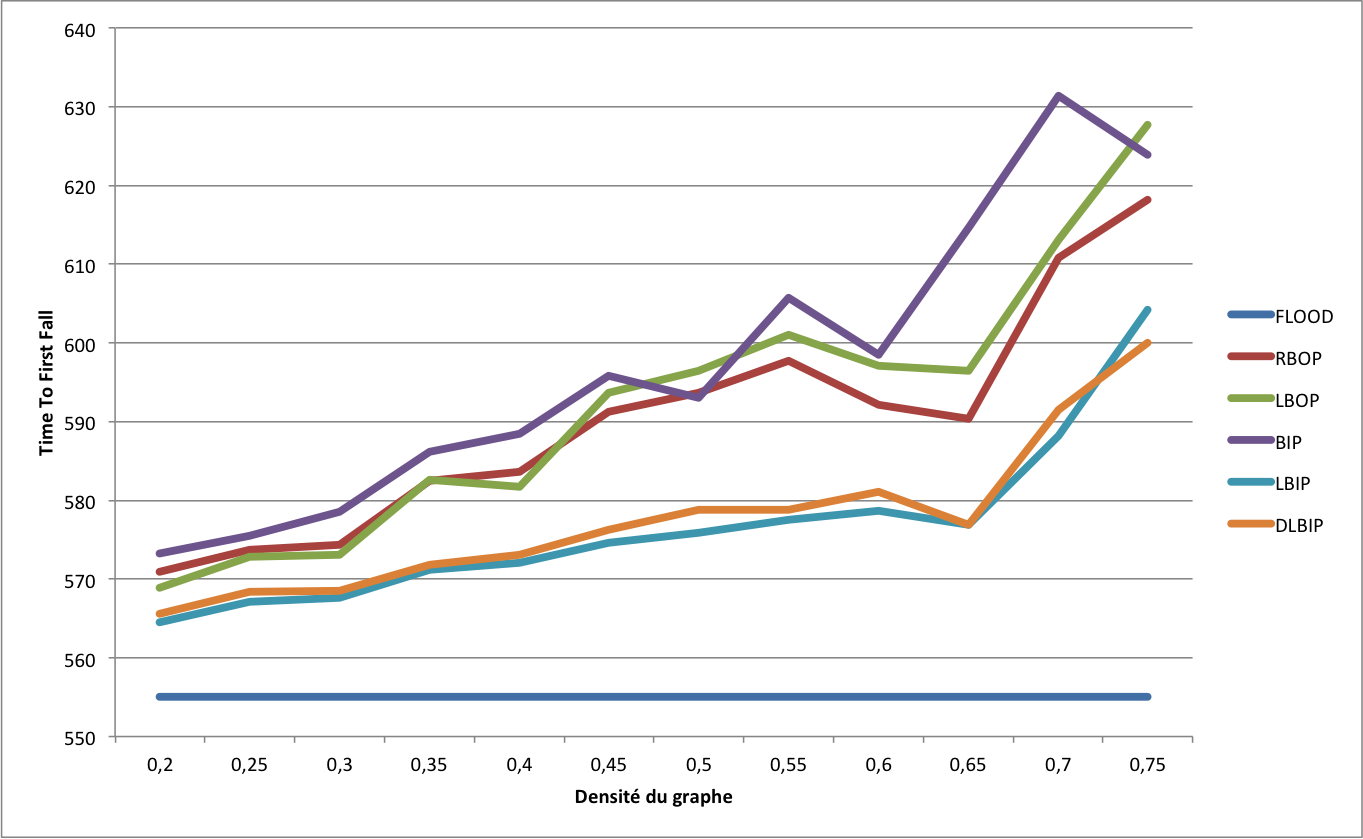
\includegraphics[scale=0.9]{Simus/ttff_4_10p6}
\end{bigcenter}


\subsubsection{PerCent Node}
\begin{bigcenter}
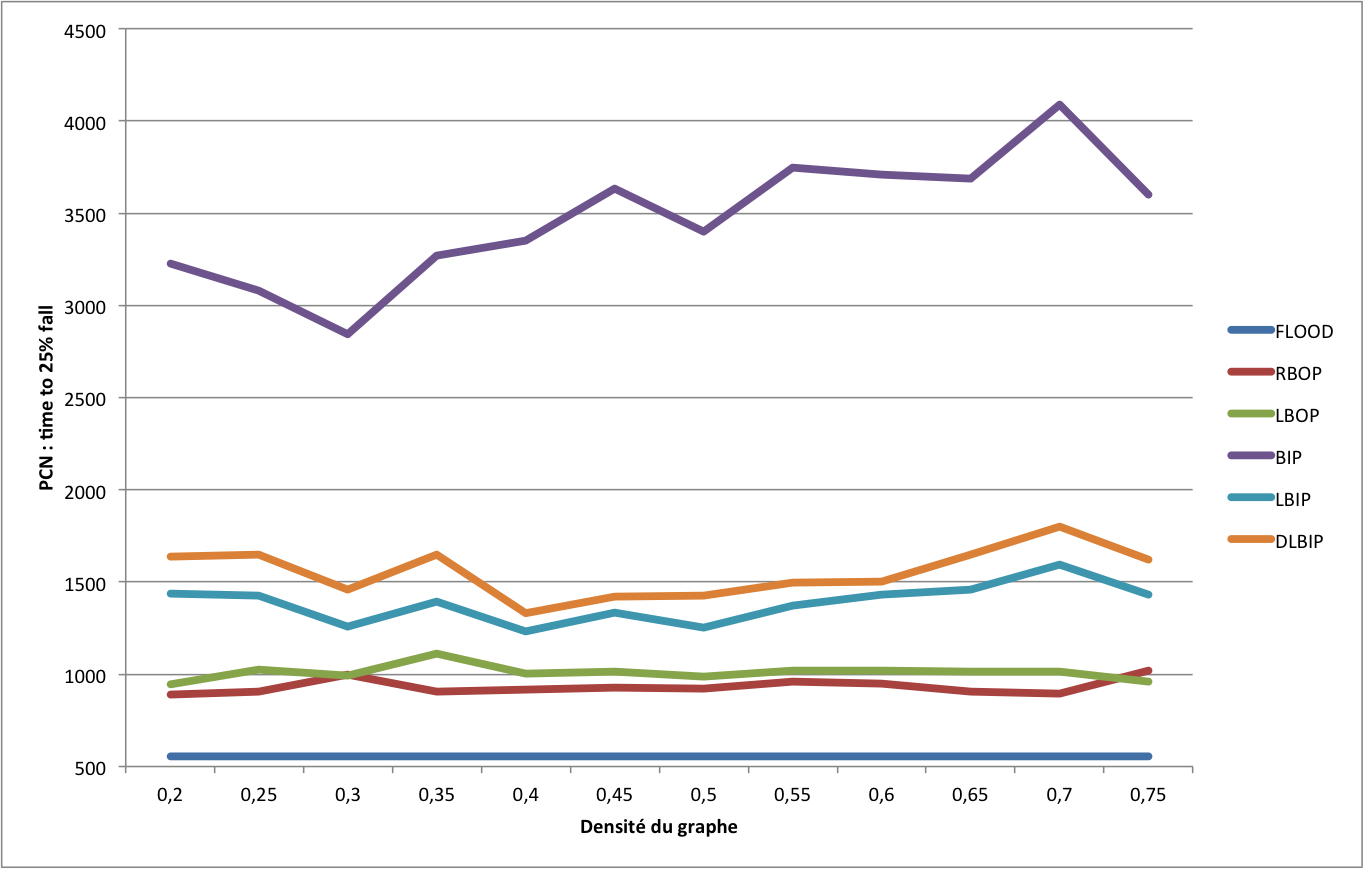
\includegraphics[scale=0.9]{Simus/pcn_4_10p6}
\end{bigcenter}


\subsubsection{Lose Connectivity}
\begin{bigcenter}
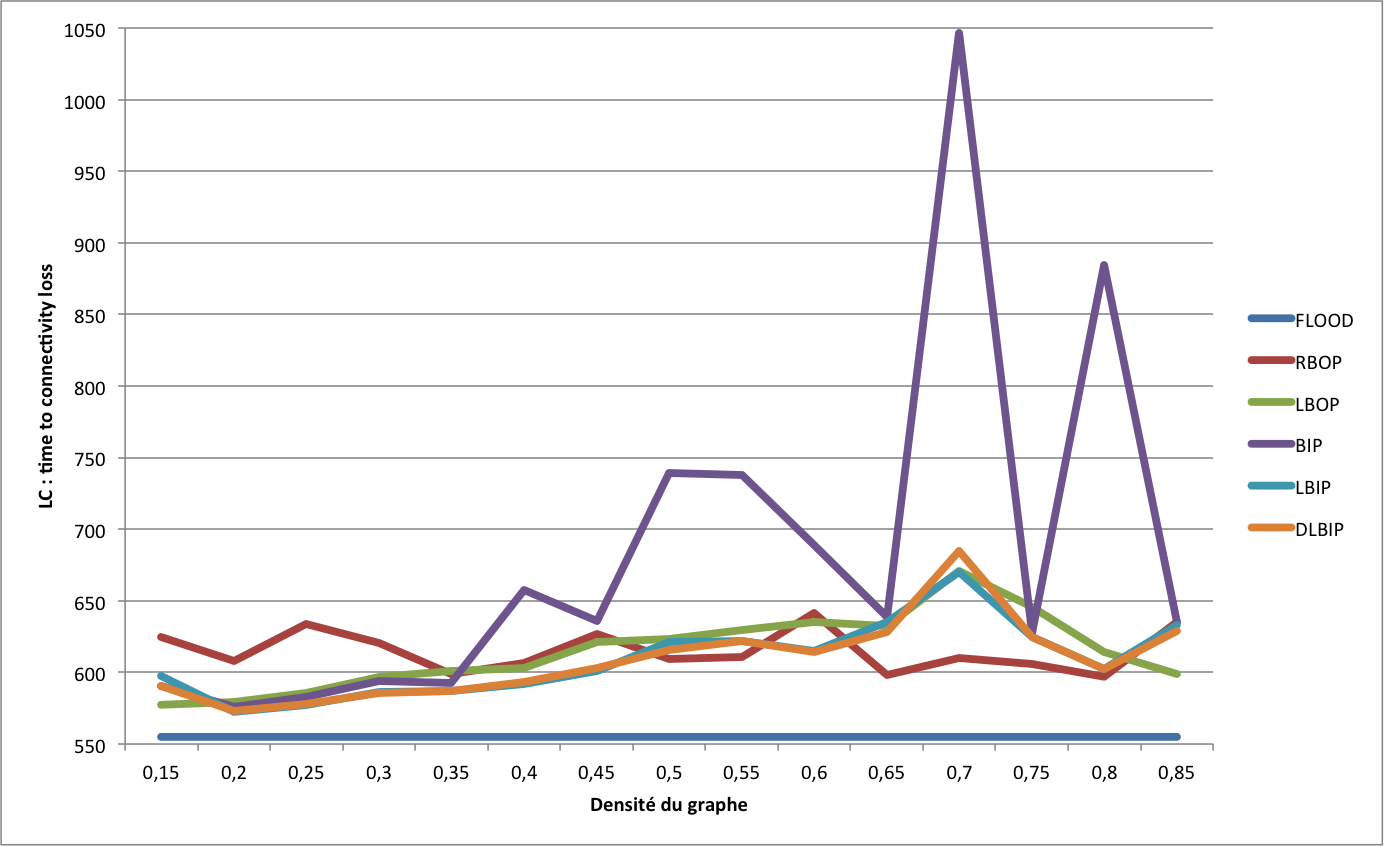
\includegraphics[scale=0.89]{Simus/lc_4_10p6}
\end{bigcenter}
